\chapter{Guía Básica de Implementación para ORPSoC}

 \section{Introdución}
Este proyecto implementa una plataforma para el desarrollo OpenRISC. Proporciona un SoC de referencia, para la prueba y el desarrollo de procesadores OpenRISC.

 \section{Descarga del ORPSoC}
La el código fuente RTL, el software de prueba y scripts de instalación pueden ser descargados del repositorio svn del proyecto OpenRISC. Los archivos pueden descargados con el siguiente comandos.

\begin{lstlisting}[breaklines]
 usuario@usuario-desktop:~/$  svn co http://opencores.org/ocsvn/openrisc/openrisc/trunk/orpsocv2
\end{lstlisting}

Después de descomprimir el archivo descargado para la instalación ORPSoC se parece a esto ~\ref{fig:esquema} 

\begin{figure}[h!]
 \begin{center}
  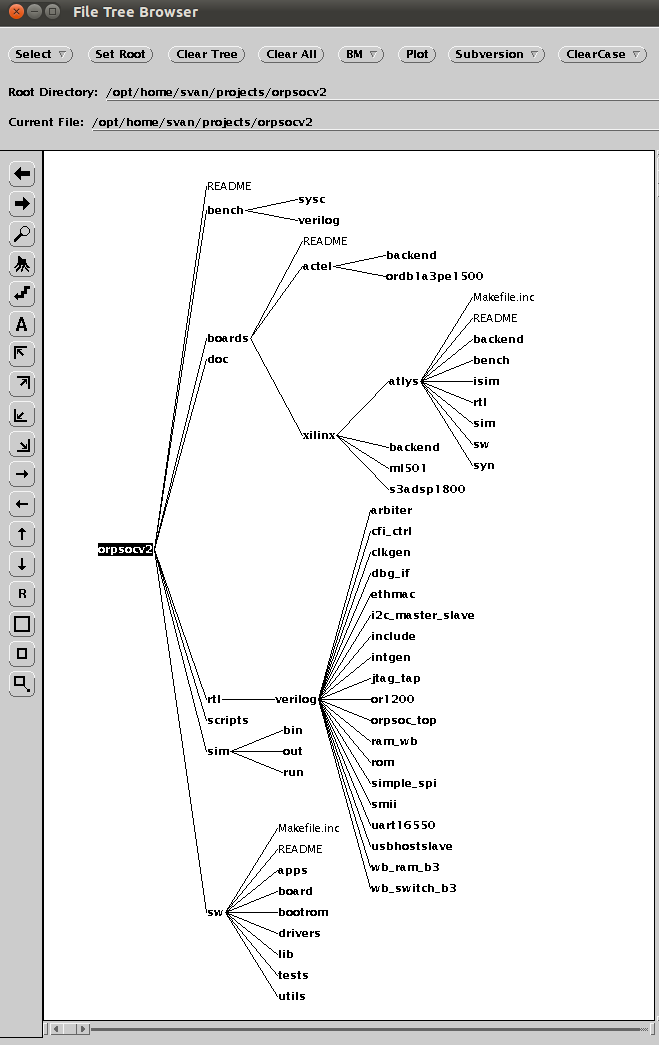
\includegraphics[width=0.8\textwidth,keepaspectratio=true]{./images/proyectoorpsoc}
  \caption{Esquema del Proyecto ORPSoC }
  \label{fig:esquema}
 \end{center}
\end{figure}

 \section{Instalación de herramientas}
 \subsection{Instalación de herramientas GNU}

Los programas deben ser instalados en el directorio / opt. Utilice los siguientes comandos para descomprimir y descomprimir el archivo descargado: 


 \section{Instalación de herramientas Xilinx}

Antes de realizar esto necesitamos tener instaladas correctamente las herramientas de Xilinix. Luego de la instalación debemos agregar al PATH de Linux las rutas a los binarios necesarios para realizar el proceso. 

\begin{lstlisting}[breaklines]
 usuario@usuario-desktop:~/$ source (ruta a Xilinx ISE)/settings32.sh  
\end{lstlisting}

 \section{Syntesis}
La construcción del proyecto está configurada para el uso de Makefiles. Los pasos a realizar son los siguientes:

\begin{itemize}
\item Los archivos necesarios para realizar la síntesis se encuentran en 

\begin{lstlisting}[breaklines]
(orpsoc_dir)/boards/xilinx/(board)/syn/
\end{lstlisting}

\item Limpiamos cualquier síntesis anteriormente realizada 
\begin{lstlisting}[breaklines]
usuario@usuario-desktop:(orpsoc_dir)/boards/xilinx/s3adsp1800/syn/xst/run$ make clean
\end{lstlisting}

\item Verificamos que solo existe el makefile
\begin{lstlisting}[breaklines]
usuario@usuario-desktop:(orpsoc_dir)/boards/xilinx/s3adsp1800/syn/xst/run$ ls

Makefile
\end{lstlisting}

\item Realizamos una nueva síntesis
\begin{lstlisting}[breaklines]
usuario@usuario-desktop:(orpsoc_dir)/boards/xilinx/s3adsp1800/syn/xst/run$ make all
\end{lstlisting}

\end{itemize} 

% #### Generating Xilinx PRJ file ####
% #### Generating XST file ####
% #### Generating Xilinx XCF file ####
% #### Running XST ####

\section{Place and Route}
%///////////// Place and Route ////////////////////////
Luego de la síntesis para realizar el procedimiento Place and Route (PAR) debemos ir a la carpeta
\begin{lstlisting}[breaklines]
(orpsoc_dir)/boards/xilinx/(board)/backend/par/
\end{lstlisting}
Limpiamos cualquier PAR anteriormente realizado

\begin{lstlisting}[breaklines]
usuario@usuario-desktop:(orpsoc_dir)/boards/xilinx/s3adsp1800/backend/par/run$ make clean
\end{lstlisting}

Verificamos que solo existe el makefile
\begin{lstlisting}[breaklines]
usuario@usuario-desktop:(orpsoc_dir)/boards/xilinx/s3adsp1800/backend/par/run$ ls
Makefile
\end{lstlisting}

Realizamos el proceso PAR 

\begin{lstlisting}[breaklines]
usuario@usuario-desktop:(orpsoc_dir)/boards/xilinx/s3adsp1800/backend/par/run$ make orpsoc.ncd
\end{lstlisting}
El reporte del PAR se encuentra en 
\begin{lstlisting}[breaklines]
usuario@usuario-desktop:(orpsoc_dir)/boards/xilinx/s3adsp1800/backend/par/run$ cat orpsoc.par
\end{lstlisting}

Para listar los valores de configuración con las que se esta realizando el proceso
\begin{lstlisting}[breaklines]
usuario@usuario-desktop:(orpsoc_dir)/boards/xilinx/s3adsp1800/backend/par/run$ make print-config
\end{lstlisting}

Para realizar un informe de "timing post place" 

\begin{lstlisting}[breaklines]
usuario@usuario-desktop:(orpsoc_dir)/boards/xilinx/s3adsp1800/backend/par/run$ make timingreport
\end{lstlisting}

El informe se encuentra en:

\begin{lstlisting}[breaklines]
usuario@usuario-desktop:(orpsoc_dir)/boards/xilinx/s3adsp1800/backend/par/run$ cat orpsoc.twr | less
\end{lstlisting}


 \section{Generación del .Bit}

Finalmente generamos el bitfile que contiene la configuración que debemos cargar en la FPGA.

\begin{lstlisting}[breaklines]
usuario@usuario-desktop:(orpsoc_dir)/boards/xilinx/s3adsp1800/backend/par/run$ make orpsoc.bit
\end{lstlisting}

 \section{Configuración de la FPGA}

%//////////// XC3SPROG INSTALLATION   //////////////
Para descargar el bitfile de configuración utilizamos xc3sprog y un programador basado en FTDI2232. Este hardware requiere de la herramienta 

Descargamos el código del programa
\begin{lstlisting}[breaklines]
usuario@usuario-desktop:~/$ svn checkout svn://svn.code.sf.net/p/xc3sprog/code/trunk xc3sprog-code
usuario@usuario-desktop:~/$ cd xc3sprog-code
usuario@usuario-desktop:~/$   
\end{lstlisting}
%........   TERMINAR PROCESO DE COMPILACIÓN ..... 


%//////////// DOWNLOAD THE BITSTREAM ON FPGA   //////////////

Luego de conectar el programador en el conector J4. Chequeamos el funcionamiento escaneando la cadena JTAG
\begin{lstlisting}[breaklines]
usuario@usuario-desktop:~$ sudo (ruta a xc3sprog)/xc3sprog  -c ftdi -j
usuario@usuario-desktop:(orpsoc_dir)/boards/xilinx/s3adsp1800/backend/par/run$ sudo (ruta a xc3sprog)/xc3sprog  -c ftdi  orpsoc.bit 
\end{lstlisting}

 \section{Descarga del BITSTREAM a la SPI }

%//////////// DOWNLOAD THE BITSTREAM ON SPI   //////////////
Inicialmente descargamos el bitfile provisto en la carperta
\begin{lstlisting}[breaklines]
xc3sprog/bscan_files
\end{lstlisting} 
 que configura la fpga para actuar como intermediario ante la FLASH SPI y así lograr grabar en la misma.
\begin{lstlisting}[breaklines]
usuario@usuario-desktop:(orpsoc_dir)/boards/xilinx/s3adsp1800/backend/par/run$ sudo (ruta a xc3sprog)/xc3sprog  -c ftdi (ruta a xc3sprog)/bscan_spi/xc3sd1800-fg676.bit 
\end{lstlisting} 

Ahora podemos descargar el bitstream a la FLASH SPI mediante 
\begin{lstlisting}[breaklines]
usuario@usuario-desktop:(orpsoc_dir)/boards/xilinx/s3adsp1800/backend/par/run$ sudo (ruta a xc3sprog)/xc3sprog  -c ftdi  -I orpsoc.bit 
\end{lstlisting}